%!TEX root = ../scivis_lbaakman_bvanloon.tex
\chapter{Gradients} % (fold)
\label{cha:gradients}
In the previous chapters we covered the various datasets in the simulation; the fluid density, fluid velocity, and the force field. In this chapter we discuss how two vector fields are created using the existing data: the fluid density gradient and the fluid velocity gradient. Gradients are multi-variable generalization of derivatives and are a function of change on the associated dataset. These vector fields indicate the direction of greatest change and the amount of change in that direction. Since the gradients are not directly represented, they have to inferred from the existing data.

\section{Calculating Gradients} % (fold)
\label{sec:calculating_gradients}
The fluid density for each vertex of the visualization grid is computed with the process discussed in \cref{cha:glyphs}.The gradient of a point on the grid is calculated by looking at the difference between the values of vertices of the cell containing that point and linear interpolating this difference based on the position of the point in the cell. Similar to the interpolation of the vector data, the gradient vector can be interpolated by interpolating the $x$ and $y$ components independently, thus: 
\begin{align*}
\Delta \begin{bmatrix}x\\y \end{bmatrix} = \begin{bmatrix}\Delta x\\\Delta y \end{bmatrix} .
\end{align*}

Given the scalar values at the four cell vertices: $\text{UL}$ for the upper left, $\text{UR}$ for the upper right, $\text{BL}$ for the bottom left, and $\text{BR}$ for the bottom right vertex the gradient of point $p$ is calculated according to:
\begin{align*}\label{eq:gradient}
	\Delta x = (1 - p_y) * \frac{BR - BL}{C_w} +
      p_y * \frac{UR - UL}{C_w}\\
	\Delta y = (1 - p_x) * \frac{UL - BL}{C_h} +
      p_y * \frac{UR - BR}{C_w}
\end{align*}
This method can be used for both the gradient of the fluid density as well as for the gradient of the fluid velocity magnitude.

\section{Visualization of Gradients} % (fold)
\label{sec:visualization_of_gradients}
Since the gradients are vector data, containing both direction and magnitude, they are best visualized using the glyphs presented in \cref{cha:glyphs}. \Cref{fig:gradients} shows the gradient vector field visualized with glyphs super imposed on the scalar visualization of the fluid density. \Cref{fig:gradients:density} clearly shows that the gradient points in the direction of the highest rate of change.

The fluid velocity gradient displayed in \cref{fig:gradients:velocity} appears to be pointing in the opposite direction of the fluid density gradient. Thus fluid moves away from locations which have a relative high density. This effect is even better noticeable when we zoom in on an area with high fluid density, see \cref{fig:gradients:zoom}.
\begin{figure}[tbh]
	\centering
	\begin{subfigure}{0.45\textwidth}
		\centering
		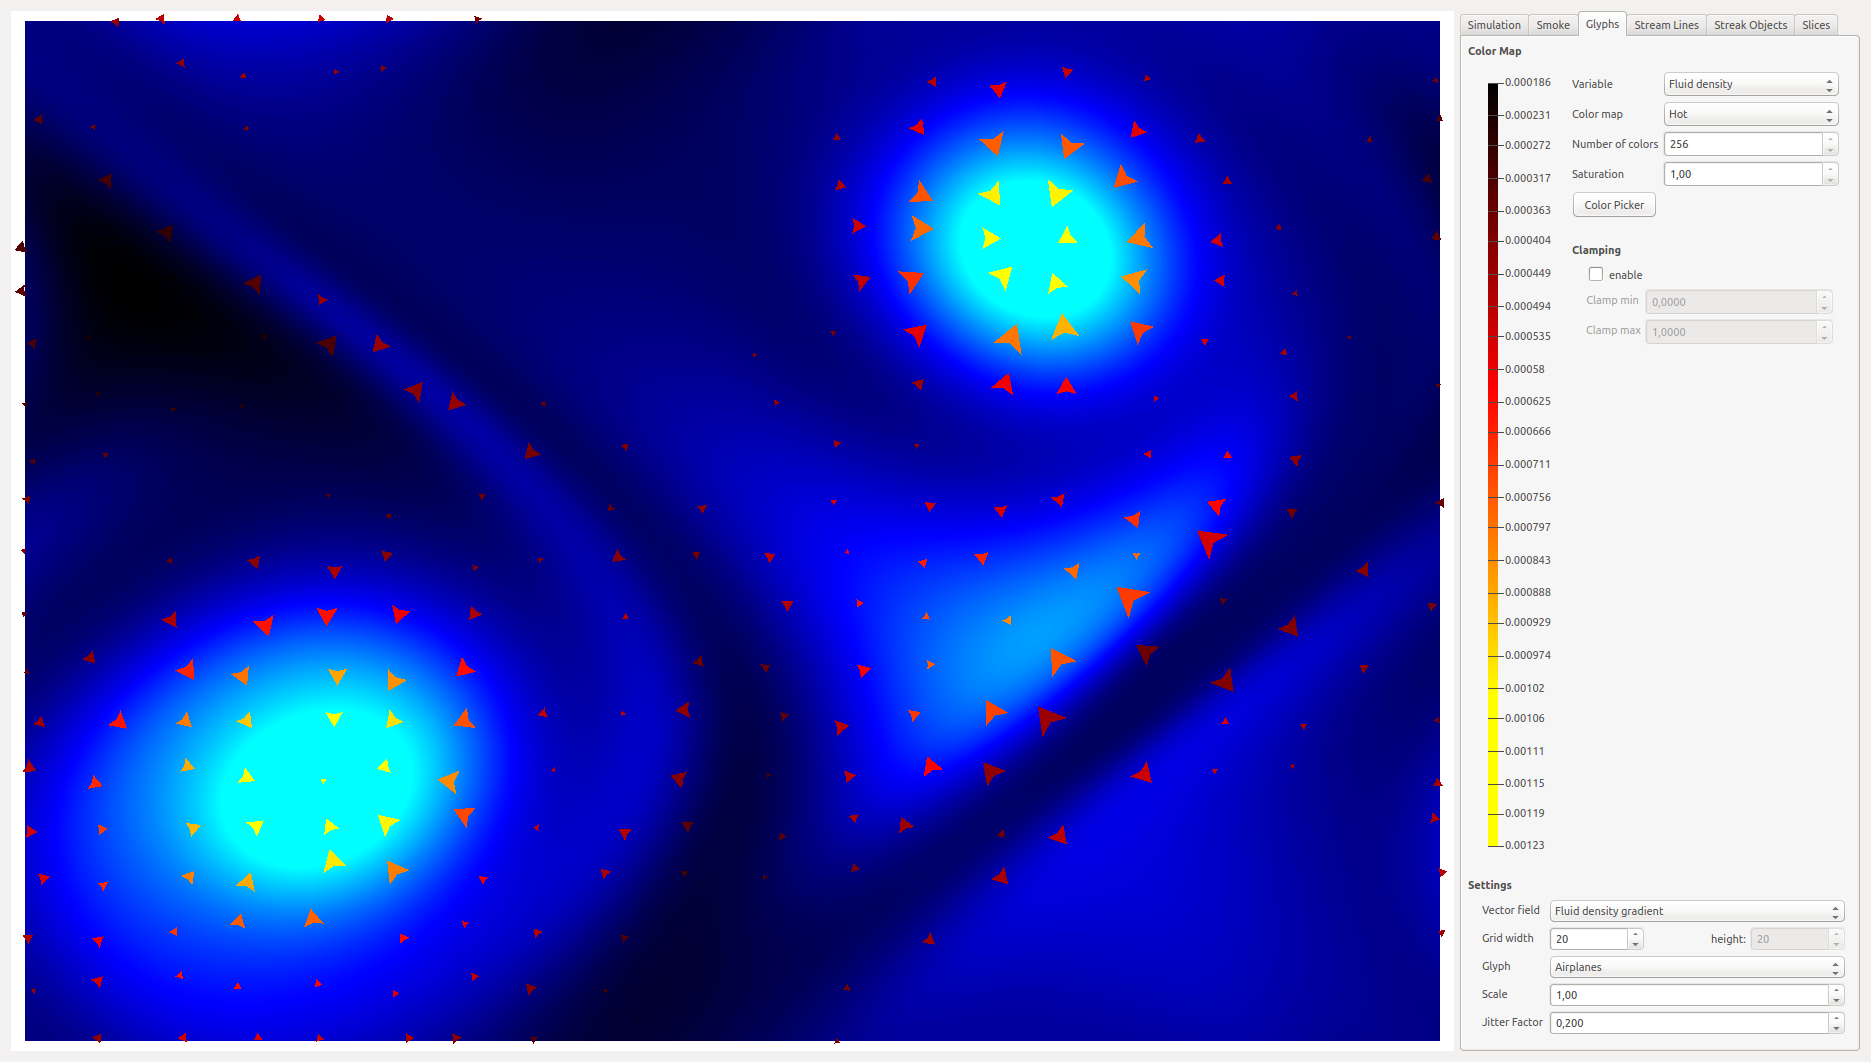
\includegraphics[width=0.9\textwidth, trim={35px 30px 430px 30px}, clip]{img/gradient/fluid_density_gradient}
		\caption{The fluid density with superimposed airplane glyphs showing the fluid density gradient.}
		\label{fig:gradients:density}
	\end{subfigure}
	\hspace{30px}
	\begin{subfigure}{0.45\textwidth}	
		\centering
		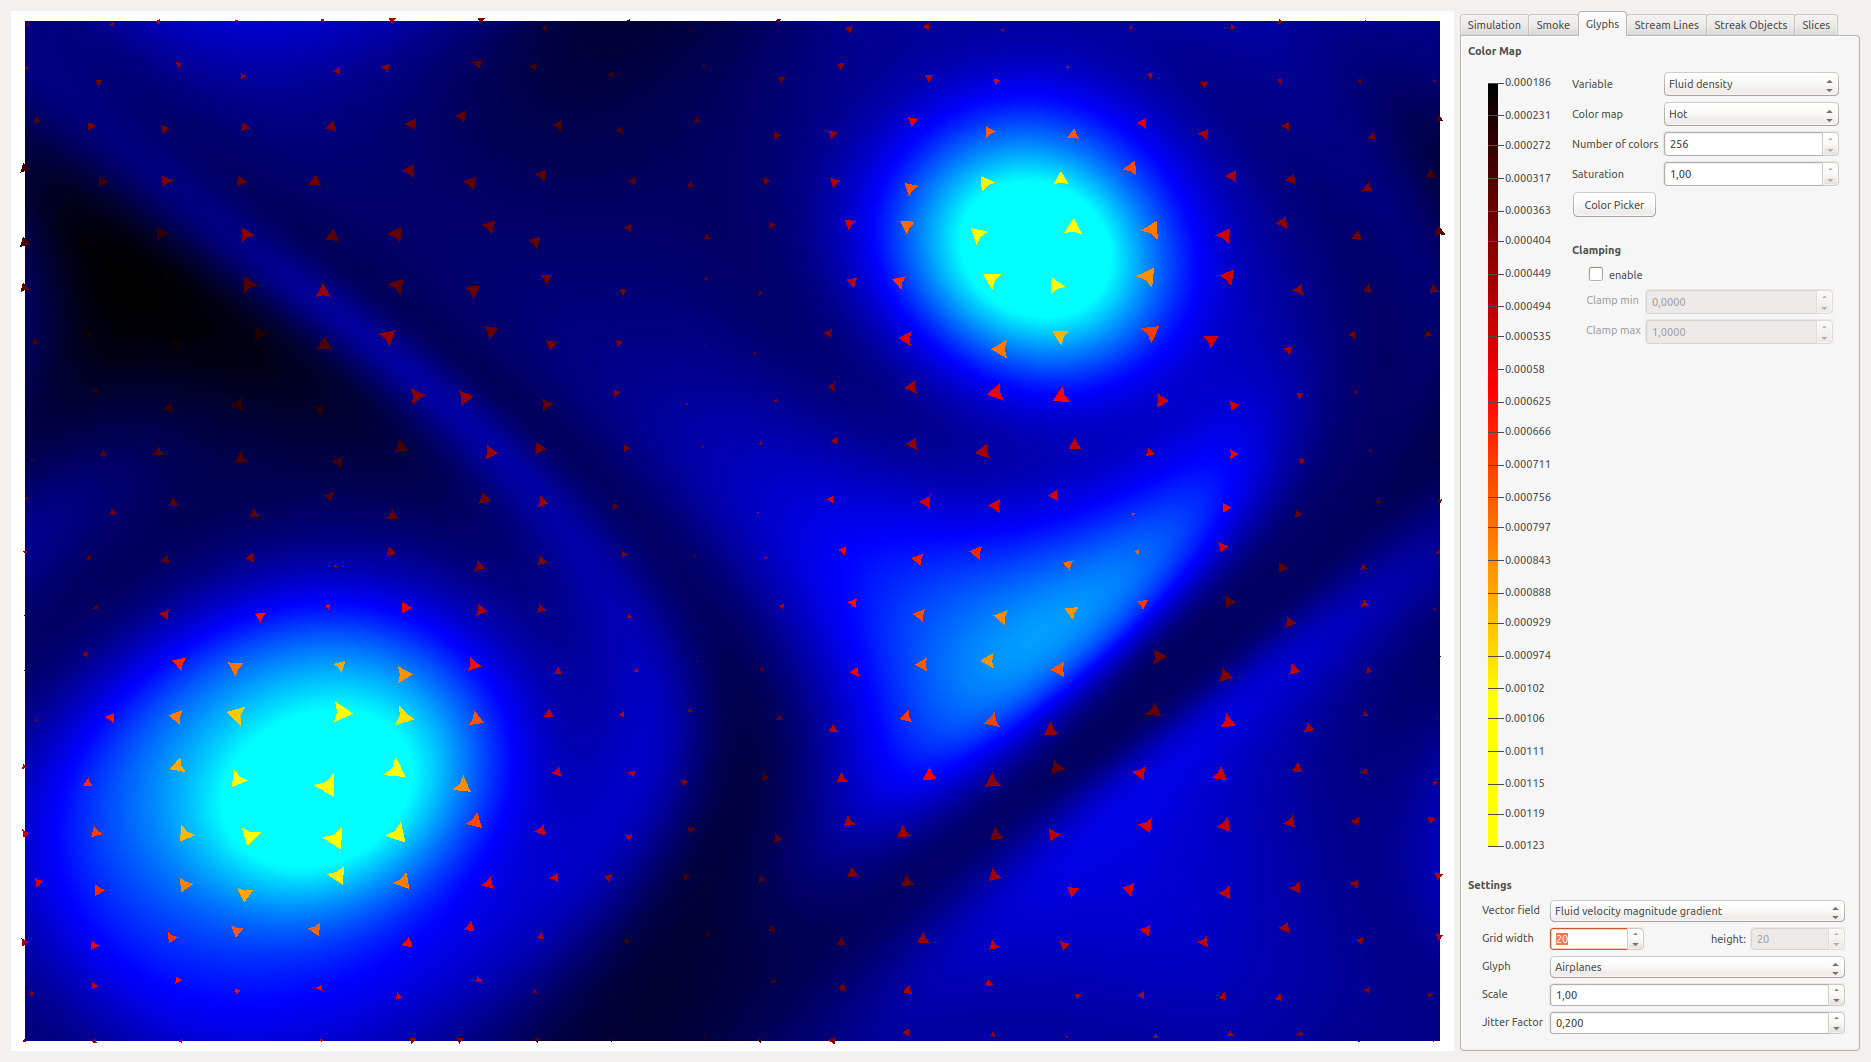
\includegraphics[width=0.9\textwidth, trim={35px 30px 430px 30px}, clip]{img/gradient/fluid_velocity_gradient}
		\caption{The fluid density with superimposed airplane glyphs showing the fluid velocity gradient.}
		\label{fig:gradients:velocity}
	\end{subfigure}
	\caption{The difference between the fluid velocity gradient and fluid density gradient. Both visualizations have the fluid density as background using the cold colormap and use the heat colormap for the glyphs. Both visualization use airplane glyphs on a $20 \times 20$ grid using a jitter-factor of 0.2.}
	\label{fig:gradients}
\end{figure}

\begin{figure}[tbh]
	\centering
	\begin{subfigure}{0.45\textwidth}
		\centering
		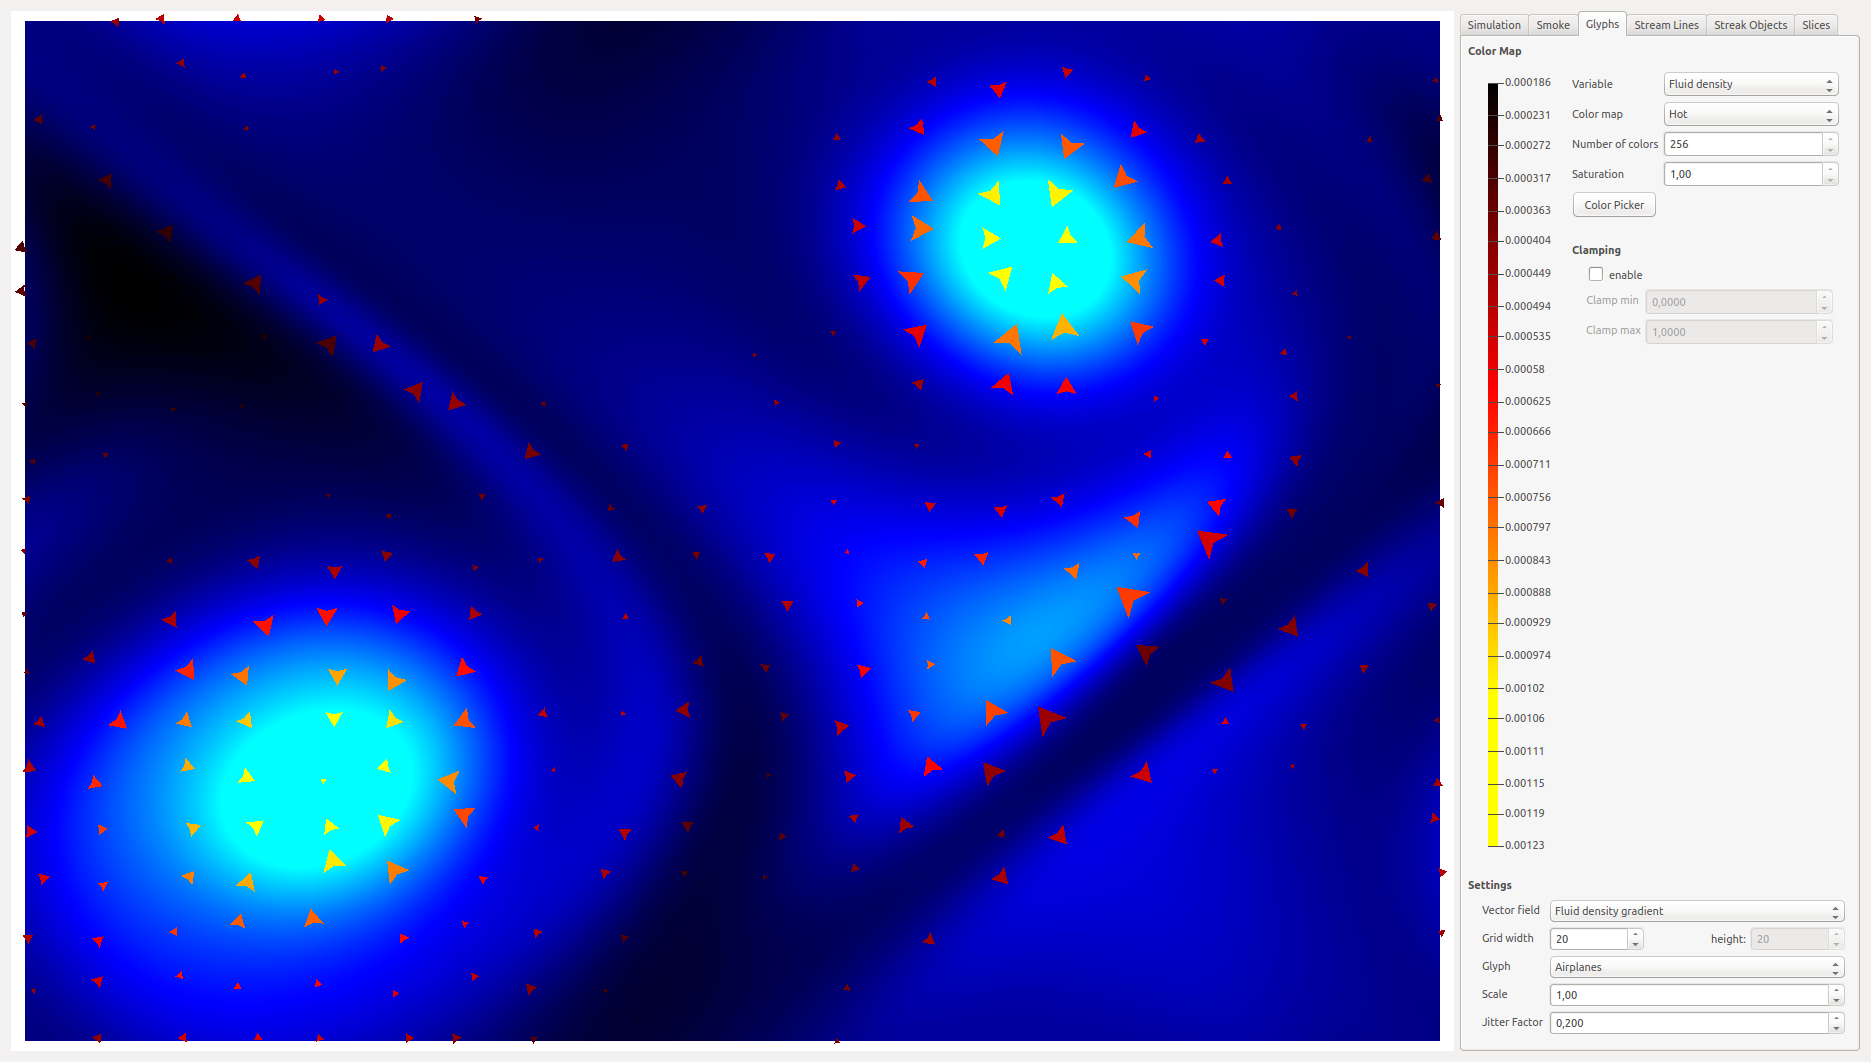
\includegraphics[width=0.9\textwidth, trim={35px 30px 1076px 500px}, clip]{img/gradient/fluid_density_gradient}
		\caption{Fluid density gradient shown in \cref{fig:gradients:density}, zoomed in on an area with max density.}
		\label{fig:gradients:zoom:density}
	\end{subfigure}
	\hspace{30px}
	\begin{subfigure}{0.45\textwidth}	
		\centering
		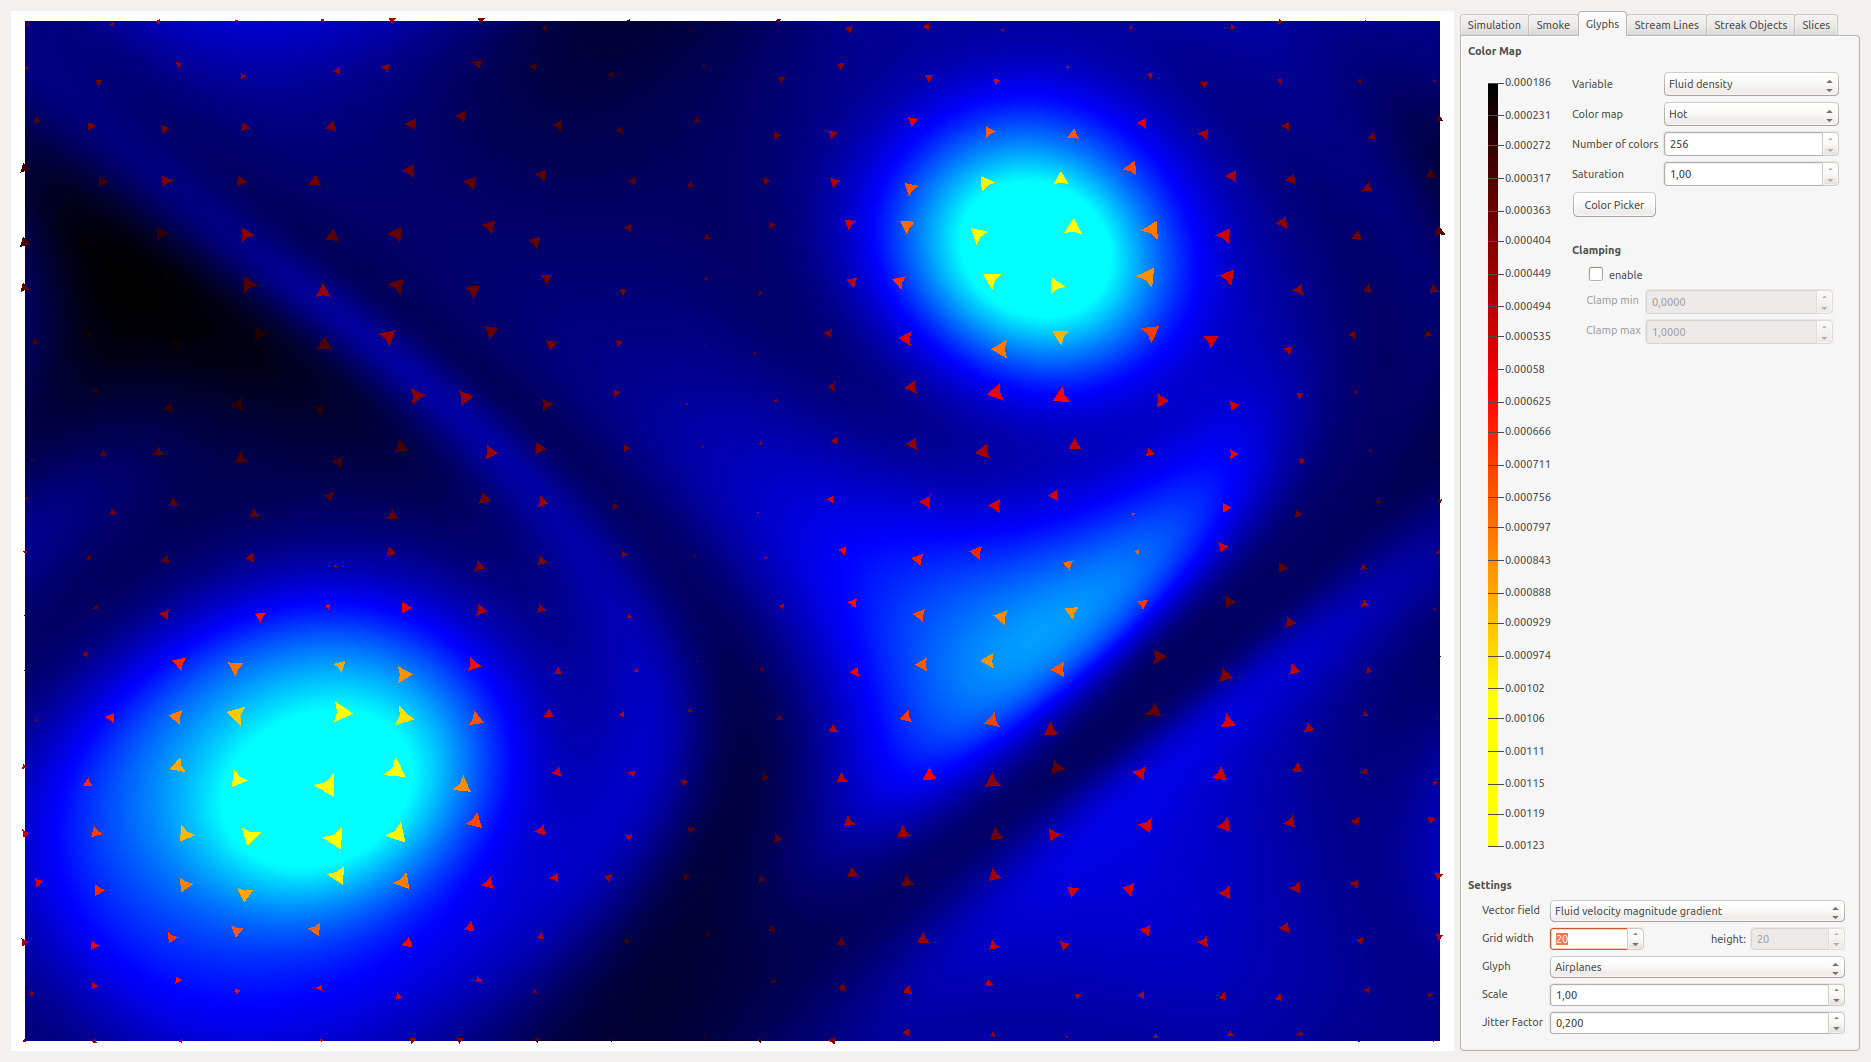
\includegraphics[width=0.9\textwidth, trim={35px 30px 1076px 500px}, clip]{img/gradient/fluid_velocity_gradient}
		\caption{Fluid density gradient shown in \cref{fig:gradients:velocity}, zoomed in on an area with max density.}
		\label{fig:gradients:zoom:velocity}
	\end{subfigure}
	\caption{A zoomed in version of \cref{fig:gradients} showing one of the areas with the highest density.}
	\label{fig:gradients:zoom}
\end{figure}